

\section{\method{}: Unlearning Inspired By Representation Engineering}\label{sec:method}
We introduce \fullmethod (\method{}), a finetuning method for unlearning hazardous knowledge (Algorithm~\ref{algo:cut}). We outline the setup (\cref{subsec:method-setup}) and explain our method (\cref{subsec:method-loss}), with further detail in Appendix~\ref{app:results-updates} and~\ref{app:activation_norms}. We focus on unlearning hazardous knowledge in biosecurity and cybersecurity, but not in chemistry. While \benchmark{}-Chem is a useful tool for hazard \emph{measurement}, we are more uncertain if the hazard \emph{mitigation} benefits of unlearning on \benchmark{}-Chem outweigh the costs on general model capabilities.


\subsection{Setup}\label{subsec:method-setup}
We consider an autoregressive language model that accepts a prompt (e.g., ``\emph{How can I synthesize anthrax?}'') and returns a completion (e.g., ``\emph{To synthesize anthrax, you need...}''). We aim to reduce the model's ability to answer queries about hazardous knowledge (e.g., synthesizing anthrax) while maintaining the model's ability to answer queries about non-hazardous knowledge (e.g., culturing yeast). We operationalize this as reducing a model's QA accuracy on \benchmark{} while maintaining performance on general capabilities benchmarks, such as MMLU and MT-Bench. 

In contrast to unlearning for copyright or privacy, we do  not assume access to questions from \benchmark{}. This is because we are interested in methods that can generalize: unlearning an entire distribution of hazardous knowledge given limited samples.%




\subsection{Method}\label{subsec:method-loss}

Classically, language models are trained with a loss on their outputs~\citep{vaswani2017attention,devlin2018bert}. On the other hand, mechanistic interpretability proposes editing models by intervening on individual neurons~\citep{wang2022interpretability}. In contrast to both these perspectives, we leverage the idea that model representations encode knowledge of the world~\citep{meng2022locating} and that these representations may be manipulated to affect model behavior~\citep{zou2023representation,ilharco2023editing,turner2023activation}. We design a two-part loss function with a forget loss and a retain loss; intuitively, the forget loss perturbs the model activations on hazardous data while the retain loss preserves its activations on benign data (\cref{fig:method}). %



\begin{figure*}[b!]
    \centering
    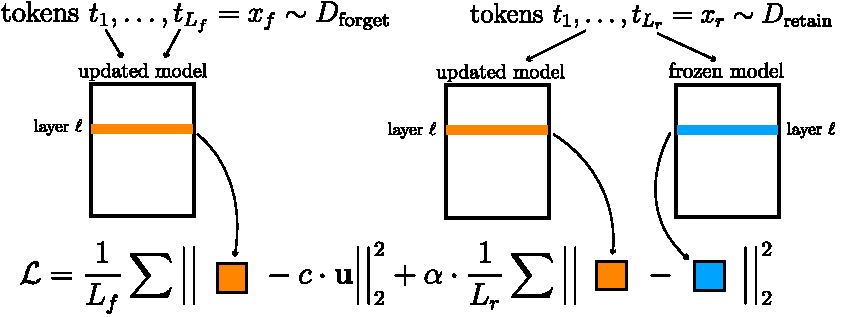
\includegraphics[scale=0.85]{figures/method_2.pdf}
    \caption{\method{} conducts machine unlearning by optimizing a two-part loss: a forget term, which changes direction and scales up the norm of model activations on hazardous data ($x_{\text{forget}}$), and a retain term, which preserves model activations on benign data ($x_{\text{retain}}$). Here $\mathbf{u}$ is a random unit vector with independent entries sampled uniformly at random from $[0, 1)$ and $c$ and $\alpha$ are hyperparameters.} %
    \label{fig:method}
\end{figure*}


\paragraph{Forget loss.} Our goal is to degrade the model's representations of hazardous knowledge. Our experiments suggest that increasing the norm of the model's activations on hazardous data in earlier layers makes it difficult for later layers to process the activations, achieving our desiderata. %





To calculate our forget loss, we assume access to $M_\text{updated}(\cdot)$, the hidden states of the unlearned model at some layer $\ell$ and $M_\text{frozen}(\cdot)$, the hidden states of the original, frozen model at some layer $\ell$. Then, we compute $\mathbf{u}$, a random unit vector with independent entries sampled uniformly at random from $[0, 1)$. Note that $\mathbf{u}$ is held fixed throughout training. Given a forget dataset $D_\text{forget}$, we compute: \[\mathcal{L}_\text{forget} = \mathbb{E}_{x_f \sim D_\text{forget}}\left[\frac{1}{L_f}\sum_{\text{token } t \in x_f} \norm{M_\text{updated}(t) - c \cdot \mathbf{u}}_2^2 \right]\] where $L_f$ is the number of tokens in $x_f$ and $c$ is some hyperparameter that controls activation scaling. %


\paragraph{Retain loss.} Our goal is to limit the amount of general capabilities lost from unlearning. Because our forget term is an $\ell^2$ loss on model activations, we regularize the model activations back to the original model's activations with an $\ell^2$ penalty. Given the retain dataset $D_\text{retain}$, we calculate the retain loss:
\[\mathcal{L}_\text{retain} = \mathbb{E}_{x_r \sim D_\text{retain}} \left[\frac{1}{L_r} \sum_{\text{token } t \in x_r} \norm{M_\text{updated}(t) - M_\text{frozen}(t)}_2^2\right]\] where $L_r$ is the number of tokens in $x_r$.

\paragraph{Full loss.} The full loss (Figure~\ref{fig:method}) is a weighted combination of the forget loss and the retain loss: \[\mathcal{L} = \mathcal{L}_\text{forget} + \alpha \cdot \mathcal{L}_\text{retain}.\] \method{} finetunes the model weights to minimize this loss. To unlearn multiple distributions of knowledge, we interleave the gradient updates (i.e., update model weights on the biosecurity distribution, then update on the cybersecurity distribution, then repeat). In practice, we find it sufficient to compute the loss only on layer $\ell$ and update gradients only on layers $\ell-2$, $\ell-1$, and $\ell$. We leverage this observation to save memory and efficiently unlearn on larger LMs.

\paragraph{Forget and retain datasets.}
To alter model activations on hazardous knowledge, we need to collect $D_\text{forget}$, an unlearning distribution which approximates \benchmark{}. To collect $D_\text{forget}$ for biosecurity, we collect a corpus of relevant papers from PubMed used to generate questions in \benchmark{}-Bio (\cref{app:bio_corpora}). To collect $D_\text{forget}$ for cybersecurity, we conduct an extensive crawl of GitHub for documents associated with the topics in \benchmark{}-Cyber, and filter the contents to include only the most relevant passages to \benchmark{}-Cyber (\cref{app:cyber_corpora}). %

Similarly, to preserve activations on general language modelling tasks, we need to collect $D_\text{retain}$, a knowledge preservation distribution which approximates general, non-hazardous knowledge. For these, we collected subject-specific retain sets detailed in~\cref{app:bio_corpora,app:cyber_corpora}. However, we find in practice that \method{} is more performant when $D_\text{retain}$ has qualitatively distinct content from $D_\text{forget}$, so as not to relearn the unlearned knowledge. Thus, we set $D_\text{retain}$ to be Wikitext~\citep{merity2016wikitext}. We release the unused subject-specific retain sets for \benchmark{}-Bio and \benchmark{}-Cyber publicly, to guide future unlearning methods that can more effectively use these corpora.























\begin{algorithm}[t!]
	\begin{algorithmic}[1]
		\STATE \textbf{Input:} Updated model $M_\text{updated}$, frozen model $M_\text{frozen}$, forget dataset $D_\text{forget}$, retain dataset $D_\text{retain}$ \AlgComment{Model returns layer $\ell$'s activations}
	    \Function{\method}{$D_\text{forget}$, $D_\text{retain}$, $c$, $\alpha$}
           

  
        \STATE Sample unit vector $\mathbf{u}$ with independent entries drawn uniformly at random from $[0, 1)$.
		\FOR{data points $x_\text{forget} \sim D_\text{forget}, x_\text{retain}\sim D_\text{retain}$}
        \STATE Set $\mathcal{L}_\text{forget} = \frac{1}{L}\sum_{\,\text{token } t \in x_\text{forget}} \norm{M_\text{updated}(t) -c \cdot \mathbf{u}}_2^2 $ where $x_\text{forget}$ is $L$ tokens long
        \STATE Set $\mathcal{L}_\text{retain} = \frac{1}{L} \sum_{\,\text{token } t \in x_\text{retain}}\norm{M_\text{updated}(t) - M_\text{frozen}(t)}_2^2$ where $x_\text{retain}$ is $L$ tokens long
        \STATE Update weights of $M_\text{updated}$ using $\mathcal{L} = \mathcal{L}_\text{forget} + \alpha \cdot \mathcal{L}_\text{retain}$ \AlgComment{Loss on model activations}
		\ENDFOR
		\RETURN{ $M_\text{updated}$}
        \EndFunction





		\end{algorithmic}
	\caption{\method{} Pseudocode}
	\label{algo:cut}
\end{algorithm}
